\section{System}
\label{sec:system}

In this work we use the formulas from Kennedy's most recent definition of PSO~\cite{4223164}.
It can be easily extended to many versions of PSO.
This version of PSO includes a constricted position update rule, a personal best update and a star topology formed by a global best update.
The constricted position update rule is
\begin{subequations}
\label{eq:pso_alg}
\begin{equation}
\label{eq:up_vel}
\begin{aligned}
v_{ij}(k+1) = &  \chi [ v_{ij}(k) 
 + \phi^{P} u^{P}_{ij}(k) (x^{P}_{ij}(k) - x_{ij}(k))\\
 & + \phi^{G} u^{G}_{ij}(k) ( x^{G}_{ij}(k) - x_{ij}(k)) ],
\end{aligned}
\end{equation}
\begin{equation}
\label{eq:up_pos}
x_{ij}(k+1) = x_{ij}(k) + v_{ij}(k+1).
\end{equation}
\end{subequations}
$ x_{ij}(k) $ represents the position of particle $ i $ in dimension $ j $ at time $ k $.
$ v_{ij}(k) $ similarly represents the velocity of particle $ i $ in dimension $ j $ also at time $ k $.
$ x^{G}_{ij}(k) $ and $ x^{P}_{ij}(k) $ are global (actually topology) and personal best positions observed by the swarm and the particle respectively. 
$ u^{G}_{ij}(k) $ and $ u^{P}_{ij}(k) $ are independent random values drawn from $ [0,1] $.
$ \chi \in ( 0, 1 ) $, $ \phi^{P} $ and $ \phi^{G} $ are algorithm parameters.
The personal best update is
\begin{equation}
\label{eq:pb_up}
x^{P}(k) = \arg \max_{ x \in \{ x(k), x^{P}(k-1) \} } f(x).
\end{equation}
The global best update is
\begin{equation}
\label{eq:gb_up}
x^{G}(k) = \arg \max_{ x \in \{ x(k), x^{G}(k-1) \} } f(x).
\end{equation}
The share of the global best makes a star topology in the swarm.

%The organization of the swarm is implemented by the star topology.
When a particle finds a new global best, it triggers a new ``global-best stagnation'' and its personal best is updated as well.
In this case, $ x(k) = x^{P}(k) = x^{G}(k) $, which means that the movement of this particle will only be driven by the inertia of the previous velocity till a new global best is found.
This particle can be viewed as a leader of this swarm.
The topology is given in Figure \ref{fig:leader_follower}.
\begin{figure}[tbph]
\centering
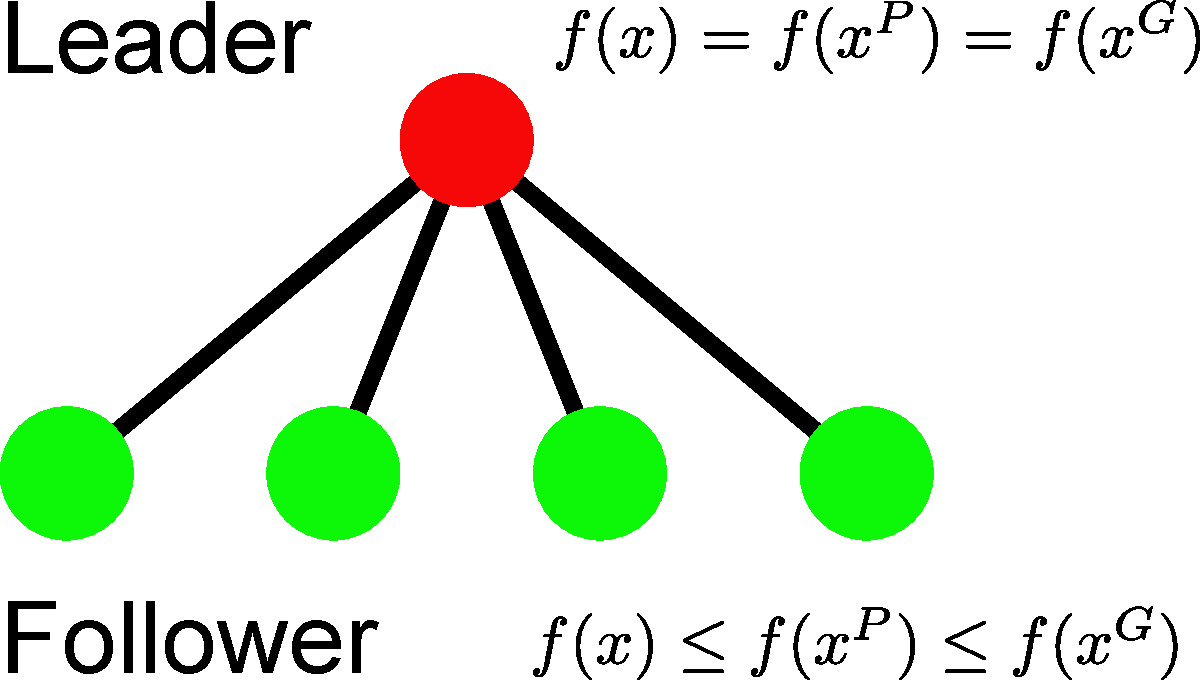
\includegraphics[width=0.5\linewidth]{./fig/leader_follower}
\caption{A leader-follower relationship.}
\label{fig:leader_follower}
\end{figure}

The star topology also supports a leader competition among the particles.
The particle that finds a new global best becomes the leader of the swarm.
The other particles are the followers, which are attracted to the leader by the impact of the global best.
By Property \ref{prop:unconverge_neq_gb}, we know that a particle will never stop moving if the personal best and the global best are inconsistent.
Thus, we can view the movements of the followers are sampling in the solution space to solve the inconsistency between its own personal best and the global best.
The input to each particle from the topology of the swarm is only the global best.

\subsection{A feedback model in a particle}

With the global best as the input, we model the behavior of a particle as a \emph{feedback system}.
%This enables analysis of PSO with stochastic factors preserved and without the stagnation assumption.
As shown in Figure \ref{fig:sys_flow}, this system is comprised of two components that form a feedback system structure.
These two components are the 
\emph{personal best update component} for the personal best ($ x^{P}_{i}(k) $), and the 
\emph{position update component} for particle position ($ x_{i}(k+1) $), which depends on the inputs $ x^{G}_{i}(k) $ and $ x^{P}_{i}(k) $ as well as the last position $ x_{i}(k) $.

\begin{figure}
\centering
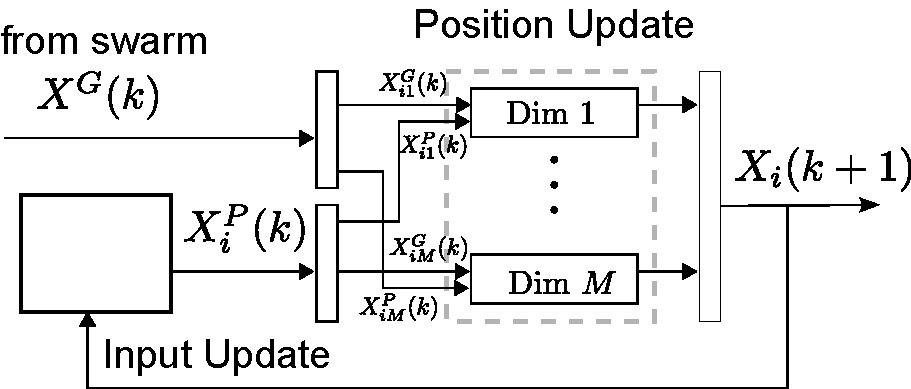
\includegraphics[width=0.85\linewidth]{./fig/sys_flow.pdf}
\caption{System structure of Particle.}
\label{fig:sys_flow}
\end{figure}

\begin{figure}
\centering
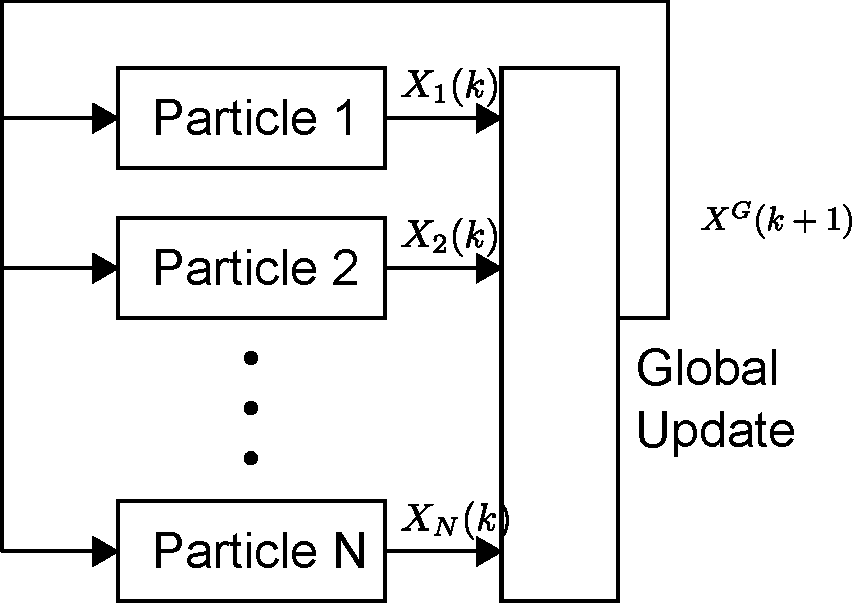
\includegraphics[width=0.6\linewidth]{./fig/pso_sys_flow.pdf}
\caption{System structure of Swarm}
\label{fig:pso_sys_flow}
\end{figure}

From \eqref{eq:pso_alg}, we can write a linear form of the position update component in one dimension.
\begin{equation}
\label{eq:pso_up_linalg_simp}
X(k+1) = A(k) X(k) + B(k) U(k)
\end{equation}
with
$ A(k) = \begin{bmatrix}
\chi & - \chi \phi^{G} u^{G}(k) - \chi \phi^{P} u^{P}(k)
\\ 
\chi & 1 - \chi \phi^{G} u^{G}(k) - \chi \phi^{P} u^{P}(k)
\end{bmatrix} $
and
$ B(k) = \begin{bmatrix}
\chi \phi^{G} u^{G}(k) & \chi \phi^{P} u^{P}(k)
\\ 
\chi \phi^{G} u^{G}(k) & \chi \phi^{P} u^{P}(k)
\end{bmatrix} $.
The system state is $ X(k) = [ v(k), x(k) - x^{R} ]^{T} $, and the system input is $ U(k) = [ x^{G}(k) - x^{R} , x^{P}(k) - x^{R} ]^{T} $
\footnote{$ x^{*} $ means an equilibrium point to the system.
When applying to the PSO, it can be a local optimum, a global optimum, or an estimated optimum.
We use it as a reference point to check the bounds.}
With a new $ x(k+1) $, the personal best update component will update the personal best $ x^{P}(k+1) $ that are fed into the position update component.

Because the position update works independently at each dimension.
When the solution space is multi-dimension, there is just a parallel connection of the position update components of all the dimensions.

The output of the personal update component is one of the inputs of the position-update component.
Take the same reference point $ x^{*} $, we can write the personal best update component as 
\begin{equation}
\label{eq:pso_input_up}
U = g(V)
\end{equation}
with $ U = [ x^{P}(k) - x^{R} ]^{T} $ 
and $ V = [ x(k) - x^{R} ] $
from \eqref{eq:pb_up}. 

Figure \ref{fig:sys_flow} shows the model structure in a particle.
Each particle has an input from the swarm, which is a global best $ x^{G} (k) $.
The position update components of all the dimensions work in a parallel structure.
The updated state $ x (k) $ will be sent into the personal best update component.
The output of the personal best component is fed back into the position update components.
With the input and output defined for a particle, we can have the system structure of the swarm in Figure \ref{fig:pso_sys_flow}.
The states of all the particles are sent into a global best update component to determine whether a new global best is found.
The global best is fed back to all the particles for the next optimization iteration.

